\section{Recurrent neural networks}

\begin{itemize}
		\item Many data sources composed of sequences: Text (of characters),
				sound (time), video (time), signals (time), ..., called
				`sequential data' or `time series'.
		\item Recurrent neural networks designed for such data
\end{itemize}

\subsection{Recap: Feed-forward networks}

Naive approach: Feed sequential data ($k$ points in $t$ sequence entries) as $k
\cdot t$ inputs to feed-forward network. But loses information about which
entries are linked by time step.

\subsection{Neurons with recurrence}

\begin{itemize}
		\item Think of neuron as recurrent cell, which influences itself and is
				fed sequential information in sequence.
		\item Alternatively think of it as sequence of linked neurons, one for
				each time step
		\item Update rules:
				\begin{itemize}
						\item New output depends on \textbf{new state}:
								$\hat{y}^t = W^T_{hy} \cdot h_t$
						\item New state depends on weighted \textbf{past state}
								and weighted \textbf{new input}: $h_t =
								f(W^T_{hh} h^{t-1} + W^T_{xh} x_t)$
				\end{itemize}
		\item Losses from all time steps combined into overall loss
\end{itemize}

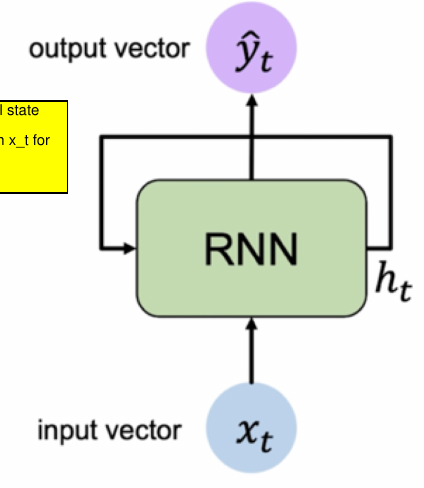
\includegraphics[width=0.5\textwidth]{09_recurrent_cell}

\subsection{Splitting data into sequences}

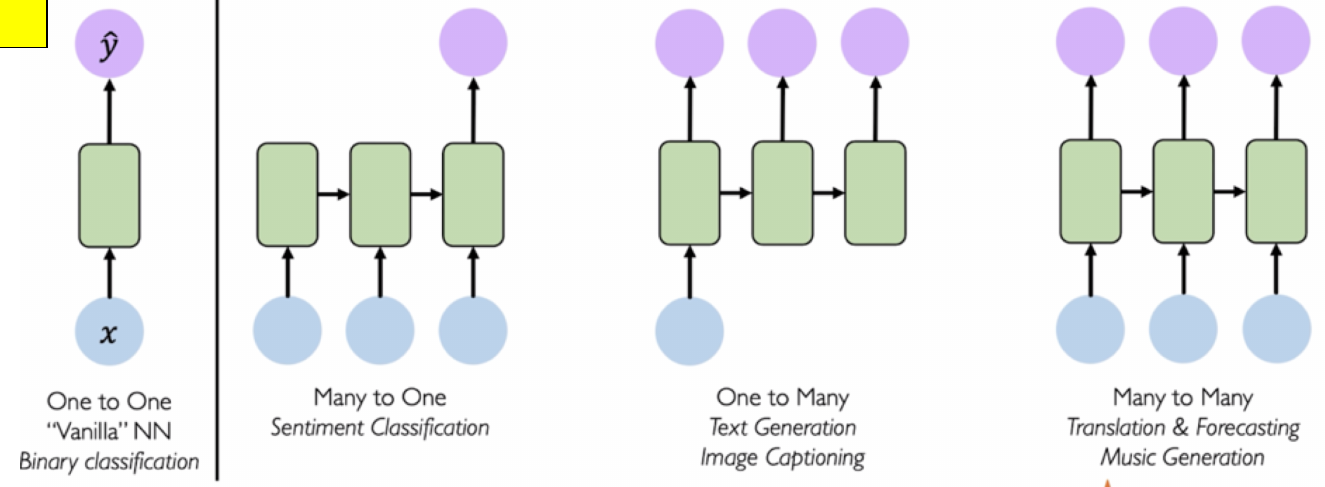
\includegraphics[width=0.7\textwidth]{09_sequential}

Challenges:
\begin{itemize}
		\item Handle variable-length sequences (e.g. sentence length)
		\item Track long-term dependencies
		\item Maintain order information
		\item Share parameters across sequence
\end{itemize}

All fulfilled by RNNs:
\begin{description}
		\item[Variable-length sequences] Map inputs to e.g. fixed-size vectors
				(based on e.g. vocabulary, or sparse vectors)
		\item[Long-term dependencies] RNN uses cell state
		\item[Order information \& shared parameters] inherent
\end{description}

\subsection{Backpropagation}

Backpropagation will go backwards through time.

Gradient contains lots of factors of state-updating weights and gradient
calculation.

\subsection{Exploding gradients}

Many values in gradient $>1$ leads to exploding gradients. Solution: Clipping.

\subsection{Vanishing gradients}

Many values in gradient $< 1$ lead to gradient converging towards $0$, no more
change in model, no more consideration for long-term factors. Multiple solutions:

\begin{itemize}
		\item ReLU as activation function
		\item Diagonal matrices for weights
		\item Gated cells (GRU, LSTM)
\end{itemize}

\subsubsection{Gated cells}

Idea: More complex recurring unit with gates to control what's passed through.
Long short term memory (LSTM) networks rely on gated cell to track information.

Standard repeating module of RNN, with black lines being addition of
weight-matrix weighted factors.

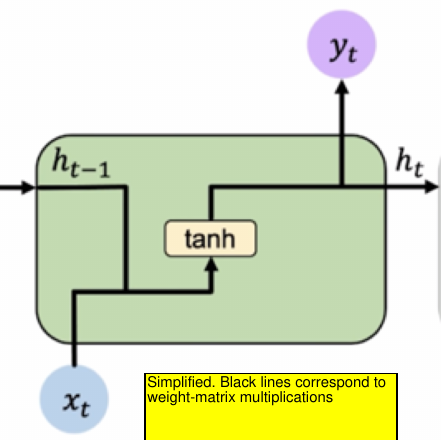
\includegraphics[width=0.5\textwidth]{09_standard_module}

For LSTM: Information added or removed through gates, which selectively let
information pass (by means of e.g. sigmoid function).

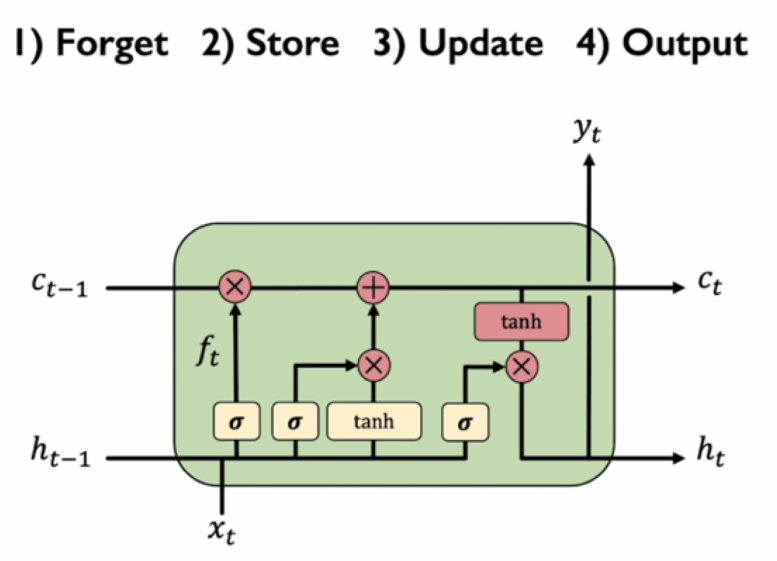
\includegraphics[width=0.5\textwidth]{09_lstm_module}

Implements:
\begin{description}
		\item[Forget] If $h_{t-1} \cdot W + x_t \cdot W$ is small, $f_t$ is
				going to be $0$ Then, $0 \cdot c_{t-1}$ will `forget' the old
				state.
		\item[Store] $\sigma(...) \cdot tanh(...)$ decides whether to store new
				state
		\item[Update] $c_t = (c_{t-1} \times forget) + (store)$ adds new
				information (if there is any worthy of storing) to state ---
				assuming the `forget' gate is not active.
		\item[Output] $h_t = \sigma(h_{t-1} \cdot W + x_t \cdot W) \times
				tanh(c_t)$ is output, also controlled by gate.
\end{description}

Also allows uninterrupted gradient flow - gradient only goes through
easy-to-derive operations.

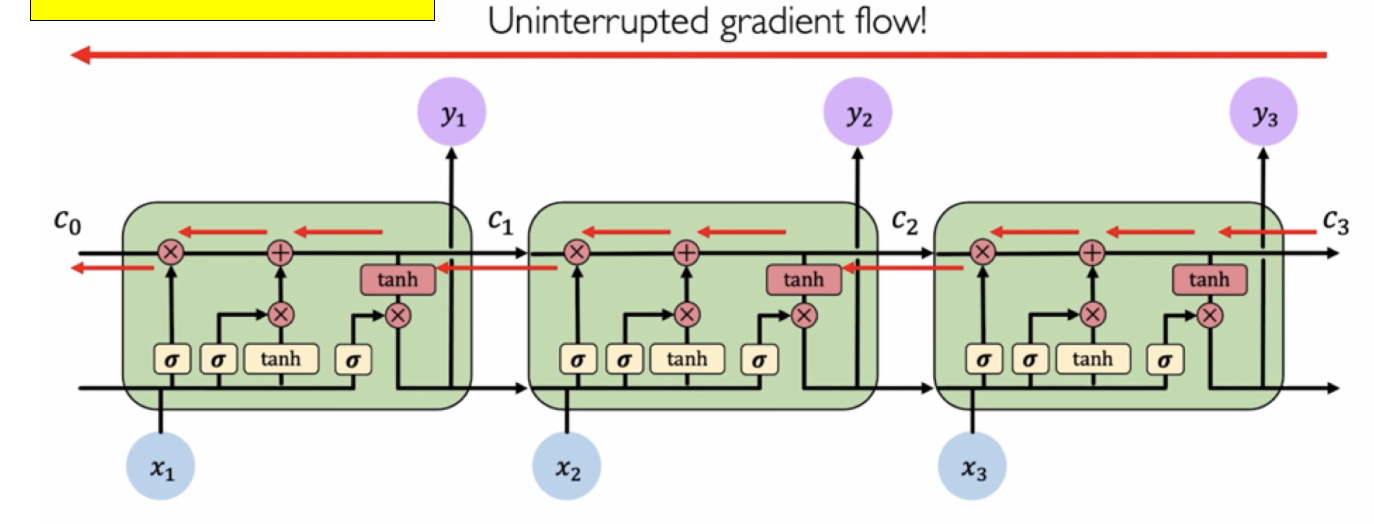
\includegraphics[width=0.7\textwidth]{09_lstm_gradient}
